% Este arquivo .tex será incluído no arquivo .tex principal. Não é preciso
% declarar nenhum cabeçalho

\section{Outras necessidades}
\subsection{Supermercados}

No centro de Barão há três supermercados: o Pague Menos (antigo Super Barão ou
``Super Ladrão'') o Pão de Açúcar e o Dalben. Ambos Pague Menos e Pão de Açúcar são
muito caros, mas o Pague Menos tem boas promoções de segunda e terça-feiras. Cada
um é melhor ou mais barato para alguma coisa. Só indo bastante em cada um é que
você pega o jeito.

\begin{figure}[h!]
    \centering
    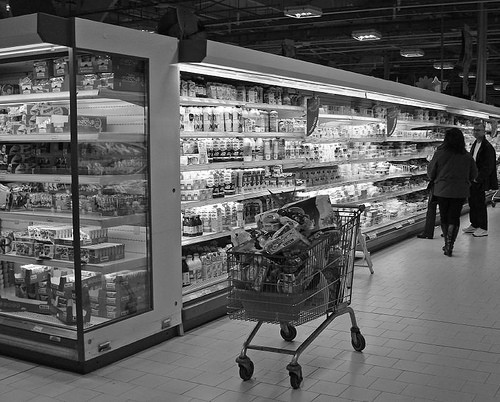
\includegraphics[scale=0.42,keepaspectratio=true]{img/imgs/9-outras_necessidades/supermercado.jpg}
\end{figure}

O Dalben é maior e geralmente tem coisas mais baratas que o Pão de Açúcar. Às
segundas e terças (no Dalben e no Pague Menos) e às terças (no Pão de Açúcar) há
preço promocional de frutas e verduras. O Dalben localiza-se no alto da Avenida
1, na entrada de Barão Geraldo. O Pague Menos funciona de segunda a sábado das 7h às
22h e aos domingos das 8h às 20h, e o Pão de Açúcar funciona de domingo
a quinta-feira das 7h às 23h, às sextas e aos sábados das 7h às 24h. Na moradia, há
outro Pague Menos e o Benatti, e no Real Parque outra loja do Pague Menos.

Há também lojas de conveniência (como as AM/PM em frente à Unicamp na Av. 1,
e no Rio das Pedras e a da Shell no fim da Avenida 2 e em frente ao Terminal,
a mais barata das quatro) que embora mais caras que os supermercados, podem funcionar
em horários alternativos ou serem mais perto de onde você mora.

Em frente ao Terminal Barão há o Recanto Bela Fruta, que não é exatamente um
supermercado, mas é o melhor lugar de Barão para comprar frutas, verduras
e legumes. Vende também algumas coisas de supermercado como pão, leite, iogurte,
Mupy etc. Neste mesmo esquema funciona o varejão Oba, que fica na avenida Santa
Isabel, perto da pizzaria Sapore. Na estrada da Rhodia, depois da Padaria Di
Capri, há a frutaria Rio das Pedras, que tem preços no nível do Pão de Açúcar
e do Pague Menos, mas é mais próximo pra quem vive na Cidade Universitária 2,
por exemplo.

Se você tiver carro, ou conhecer alguém que tenha, junte um pessoal e faça suas
compras no Tenda Atacado ou no Atacadão. Os dois são muito mais baratos que
qualquer supermercado e têm muita variedade. Ah, e nem tudo é atacado, vende
umas coisas a varejo lá também. Para chegar aos dois, saindo de Barão pelo
Tapetão, pegue a D. Pedro sentido Anhanguera. Assim que você entrar na D. Pedro,
você já vai enxergar o Atacadão, à direita. Para ir ao Tenda siga mais um pouco
na D.  Pedro e saia logo depois do CEASA à direita.

Outras opções para quem tem carro são: O Carrefour, localizado na Rodovia D.
Pedro e o Wal-Mart, que fica no Shopping Parque D. Pedro.

\subsection{Utilidades em geral}

\begin{itemize}
\item  \textbf{Ki-Água}
		\\Telefone: (19) 3289-4659
		\\Endereço: Rua Eduardo Modesto, 240

\item  \textbf{Circuito das Águas}
		\\Telefone: (19) 3289-4930
		\\Endereço: Rua Júlia Leite de Barros, 182

\item  \textbf{Água Mineral Serrana}
		\\Telefone: (19) 3289-4602
		\\Endereço: Av. Albino J. B. de Oliveira, 658

\item  \textbf{Real Gás}
		\\Telefone: (19) 3289-1786
		\\Endereço: Rua Eduardo Pereira de Almeida, 570

\item  \textbf{Genebra Gás}
		\\Telefone: (19) 3289-3622
		\\Endereço: Av. Santa Isabel

\item  \textbf{Drogaria Vitória}
		\\Telefone: (19) 3289-9926
		\\Endereço: Av. Ruberley Bueretto da Silva, 1015

\item  \textbf{Drogaria Nova Barão}
		\\Telefone: (19) 3289-6191

\item  \textbf{Rede Farmaxima}
		\\Telefone: (19) 3289-2824 / (19) 3289-4054
		\\Endereço: Av. Dr. Romeu Tortima, 255

\item  \textbf{Drogaria Sidarta}
		\\Telefone: (19) 3289-1999
		\\Endereço: Av. Prof. Atílio Martini, 190

\item  \textbf{New Laundry Lavanderia}
		\\Telefone: (19) 3289-3922
		\\Endereço: Rua Francisca Resende Merciai, 54

\item  \textbf{Desentupimento 24 horas}
		\\Telefone: (19) 3242-1249

\item  \textbf{Carpintaria São Jorge de Barão}
		\\Telefone: (19) 3289-3399
		\\Endereço: Av. Santa Isabel, 1882

\item  \textbf{CPFL (companhia de luz)}
		\\Telefone: 0800-010-1010

\item  \textbf{Sanasa (companhia de água)}
		\\Telefone: 0800-772-1195

\item  \textbf{Luigi Cabelereiro}
		\\Telefone: (19) 3288-0198

\item  \textbf{João Cabelereiros}
		\\Telefone: (19) 3289-3084
		\\Endereço: Rua Orácio Leonardi, 92

\item  \textbf{Armazém da Foto}
		\\Telefone: (19) 3289-0975

\item  \textbf{Correios -- Centro de Barão}
		\\Endereço: Av. Santa Isabel, 218 -- Centro de Barão
		\\Telefone: (19) 3288-0244

\item  \textbf{Correios -- Unicamp}
		\\Endereço: Rua Carlos Gomes, 241 -- Campus da Unicamp (próximo ao
       ginásio e Instituto de Artes)
		\\Telefone: (19) 3289-7288 / (19) 3521-7642
\end{itemize}

\subsection{Bancos}

\begin{figure}[h!]
    \centering
    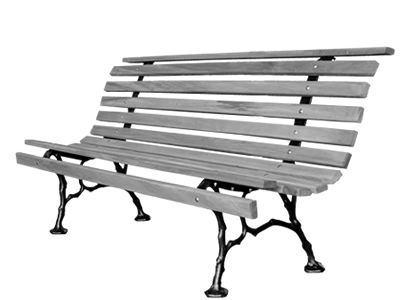
\includegraphics[scale=2.28,keepaspectratio=true]{img/imgs/9-outras_necessidades/raizmadeira.png}
\end{figure}

Bixo, agora que você está na universidade, chegou a hora de tomar vergonha na
cara e abrir uma conta no banco. A menos que você more em Campinas ou muito perto,
essa será a forma principal do papai te mandar dinheiro.

Todos os bancos oferecem algum tipo de conta universitária, que tem tarifas
reduzidas. Os documentos exigidos para abertura de conta costumam ser identidade,
CPF, comprovante de residência (conta de água, luz, telefone, gás -- pode ser do
endereço da sua cidade e no nome dos seus pais) e e comprovante de renda (pode
ser no nome dos seus pais).

Além da conta universitária, alguns bancos oferecem uma modalidade de conta
inteiramente sem custo, mas que pode ser operada apenas por meios eletrônicos,
como internet banking, caixa eletrônico, cartão de débito e crédito e telefone.
Enquadram-se nesta categoria as contas eletrônicas do Banco do Brasil e do Santander
e a iConta do Itaú.

Há várias agências bancárias dentro da Unicamp e em Barão Geraldo. Confira onde
se localizam:

\begin{itemize}
\item  \textbf{Banco do Brasil:} Há três agências: uma localizada perto da
        Reitoria, outra no centro de Barão, perto do Santander, e outra no
        centro de Barão perto do Pague Menos. Há ainda uma agência exclusiva
        para clientes Estilo próxima aos Correios da Unicamp.

\item  \textbf{Bradesco:} Agência no centro de Barão, do lado do Banco do
        Brasil e em frente do Santander. Próxima ao Terminal Barão.

\item  \textbf{Caixa Econômica Federal:} Localizada na frente do Pão de Açúcar.

\item  \textbf{Citibank:} Localizado no alto da avenida 2, próximo ao posto
        Shell.

\item  \textbf{Itaú:} Possui uma agência na Unicamp, próximo à Reitoria e à
        agência do Santander, e outra na avenida Santa Isabel, do lado da
        sorveteria. Existe também o Itaú Personnalité, próximo ao Pão de Açuar
        e ao McDonalds.

\item  \textbf{Santander:} Há quatro agêncais em Barão: duas localizadas ao lado
        da Reitoria, outra na praça do Ciclo Básico e a outra próxima ao
        Terminal Barão.
\end{itemize}

\subsection{Sebos e livrarias}

Em Barão há três sebos: O Curupira, o Cronópio e o Galpão. Geralmente você não
encontra muita coisa boa de computação neles, mas não custa procurar. O Curupira
fica na rua do Terminal, bem em frente a ele. Não é difícil achar. O Galpão fica
perto do Terminal. Saindo do terminal pela avenida marginal à Albino de
Oliveira, vire a primeira à esquerda e a segunda à direita. Funciona de segunda
à sexta até às 18h. O Cronópio fica na mesma rua do Galpão, só que bem longe,
próximo à padaria Fiori. Seguindo a Santa Isabel, vindo do Centro de Barão, vire
à esquerda na esquina que tem uma pizzaria (antes da Fiori). Vire na primeira
à esquerda e você está no Cronópio (Lá também é um restaurante barato
e gostoso).

Na Unicamp há a livraria Toledo, que fica na Faculdade de Educação (Pedago), tem
pouca coisa de Computação lá, mas sempre tem alguma coisa de Matemática. Também
há a livraria da Unicamp (no IEL), tem preços bons mas não tem quase nada de
Exatas. Já a Livraria da Química tem livros de exatas, e geralmente eles
conseguem importar a um preço bom. Outras livrarias são a Fnac (no Shopping D.
Pedro), a Saraiva e a Cultura (no Shopping Iguatemi) e a Siciliano (no Shopping
Galeria).

Mais uma dica: Antes de comprar um livro, veja se você vai usar muito ele, se
não tem bastante na biblioteca, se algum veterano legal não pode te emprestar ou
te vender, ou se não rola tirar xerox. Você compra livro só se você precisar
e/ou quiser muito. Caso vá comprar, atente para livrarias virtuais, que podem
ter preços muito menores (pesquise sempre no Buscapé
(\url{buscape.com.br})) e emitem boletos para você pagar no banco.
Em alguns casos, a livraria da Editora (localizada no piso térreo da BC) pode
trazê-lo por um preço menor ainda -- consulte sempre!

Uma última dica: Não compre o livro de G.A. (MA141). Estude pelo Stewart II
(livro de Cálculo II), pelo Steinbruch ou pelo livro do Paulo
Boulos. Os três são muito melhores que ele. Se você quiser os exercícios para
estudar para os testes pegue na internet ou tire xerox. Use os outros livros
para estudar.

\begin{figure}[h!]
    \centering
    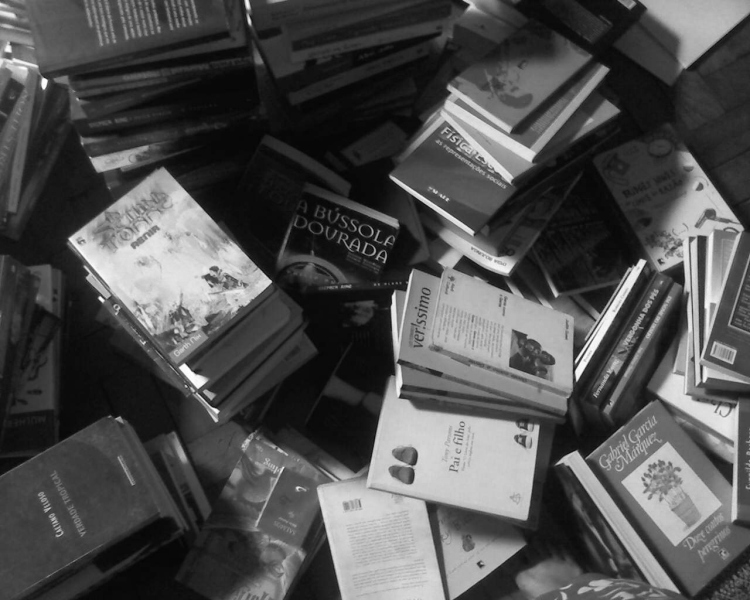
\includegraphics[scale=0.29, keepaspectratio=true]{./img/imgs/9-outras_necessidades/-068.jpg}
\end{figure}


\begin{itemize}
\item   \textbf{Sebo Curupira}
		\\Endereço: Av. Albino J. B. de Oliveira, 980
		\\Telefone: (19) 3289-7522

\item   \textbf{Sebo Galpão}
		\\Endereço: Rua Francisco Barros Filho, 16
		\\Telefone: (19) 3289-2044

\item   \textbf{Sebo Valise de Cronópio}
		\\Endereço: Rua Francisco de Barros Filho, 426
		\\Telefone: (19) 3289-0028
\end{itemize}

\subsection{Bicicletarias}

\begin{itemize}
\item   \textbf{Bicicletaria Barão}
		\\Endereço: Av. Santa Isabel, 446
		\\Telefone: (19) 3249-0449

\item   \textbf{Rei do Pedal}
		\\Endereço: Av. Santa Isabel, 74
		\\Telefone: (19) 3289-9258

\item   \textbf{Via Bike}
		\\Endereço: Av. Albino J. B. de Oliveira, 1074
		\\Telefone: (19) 3289-9888
\end{itemize}

\subsection{Escolas de idiomas}

\begin{itemize}
\item   \textbf{CCAA}
		\\Endereço: Rua Prof. Luciano Venere Decourt, 290
		\\Telefone: (19) 3249-0202
		\\E-mail: \email{barao@ccaa.com.br}
		\\Site: \url{ccaa.com.br/barao}

\item   \textbf{CCBEUC -- Centro Cultural Brasil Estados Unidos -- Campinas}
		\\Endereço: Av. Dr. Romeu Tortima, 531
		\\Telefone: (19) 3249-0275
		\\E-mail: \email{admbg@ccbeuc.com.br}
		\\Site: \url{ccbeuc.com.br}

\item   \textbf{CNA}
		\\Endereço: Av. Dr. Romeu Tortima, 553
		\\Telefone: (19) 3289-4700
		\\Fax: (19) 3289-4700
		\\E-mail: \email{baraogeraldo@cna.com.br}
		\\Site: \url{cna.com.br/baraogeraldo}

\item   \textbf{HAVAD}
		\\Endereço: Av. Dr. Romeu Tortima, 522
		\\Telefone: (19) 3288-0012
		\\Fax: (19) 3249-0488
		\\E-mail: \email{havad@havad.com.br}
		\\Site: \url{havad.com.br}

\item   \textbf{In Touch}
		\\Endereço: Rua Antônio Augusto de Almeida, 517 -- Cidade Universitária
		\\Telefone: (19) 3289-3481
		\\E-mail: \email{secretaria@intouch.art.br}
		\\Site: \url{www.intouch.art.br}

\item   \textbf{INOVA -- Escola de Inglês}
		\\Endereço: Av. Dr. Romeu Tortima, 391
		\\Telefone: (19) 3288-0071
		\\E-mail: \email{fale@inovalinguas.com.br}
		\\Site: \url{inovalinguas.com.br}

\item   \textbf{Real Time}
		\\Endereço: Rua Agostinho Páttaro, 47 (esquina com a do praça do coco)
		\\Telefone: (19) 3289-6240

\item   \textbf{Wizard}
		\\Endereço: Rua João Batista Antonioli, 90
		\\Telefone: (19) 3289-6199
		\\Site: \url{wizard.com.br}

\item   \textbf{Yazigi}
		\\Endereço: Av. Dr. Romeu Tortima, 500
		\\Telefone: (19) 3249-2375
		\\Site: \url{yazigi.com.br}
\end{itemize}

\subsection{Igrejas}

\begin{itemize}
\item   \textbf{IBCU -- Igreja Batista da Cidade Universitária}
		\\Endereço: Rua Tenente Alberto Mendes Jr., 5
		\\Telefone: (19) 3289-4501
		\\E-mail: \email{jovens@ibcu.org.br}
		\\Site: \url{ibcu.org.br}

\item   \textbf{IBBG -- Igreja Batista de Barão Geraldo}
		\\Endereço: Rua Luiz Vicentim, 284
		\\Telefone: (19) 3289-1793

\item   \textbf{IPBG -- Igreja Presbiteriana de Barão Geraldo}
		\\Endereço: Rua Francisco Andreo Aledo, 141 (próximo à praça do coco e moradia)
		\\Telefone: (19) 3289-3239

\item   \textbf{Igreja do Nazareno Betânia}
		\\Endereço: Rua Manoel Antunes Novo, 98
		\\Telefone: (19) 3289-7379

\item   \textbf{Assembleia de Deus -- Ministério de Belém}
		\\Endereço: Rua Júlia Leite de Barros, 54 (próximo à moradia da Unicamp)
		\\Telefone: (19) 3249-0035
		\\Site: \url{adbarao.com.br}

\item   \textbf{Paróquia Santa Isabel}
		\\Endereço: Rua Benedito Alves Aranha, 226
		\\Telefone: (19) 3289-1101 / (19) 3289-2323
		\\Site: \url{www.paroquiasantaisabel.org.br}

\item   \textbf{Comunidade do Estudante Universitário}
		\\Endereço: Rua Dr. Ruberlei Boaretto da Silva, 785
		\\E-mail: \email{ceu.campinas@gmail.com}
\end{itemize}

\subsection{Postos de combustível}

\begin{itemize}
\item   \textbf{Auto Posto Campineira}
		\\Endereço: Av. Albino J. B. de Oliveira, 1480
		\\Telefone: (19) 3289-5991

\item   \textbf{Auto Posto Barbieri de Barão Geraldo}
		\\Endereço: Av. Albino J. B. de Oliveira, 1001 (próximo ao terminal)
		\\Telefone: (19) 3289-1917 / (19) 9768-6713

\item   \textbf{Centro Automotivo Cidade Universitária LTDA}
		\\Endereço: Av. Dr. Romeu Tortima, 1541
		\\Telefone: (19) 3289-8457 / (19) 3289-9934 / (19) 3289-9199

\item   \textbf{Transo Combustíveis LTDA}
		\\Endereço: Av. Santa Isabel, 1030 (próximo à moradia)
		\\Telefone: (19) 3289-1012

\item   \textbf{Esso Auto Posto Futuro}
		\\Endereço: Av. Albino J. B. de Oliveira, 360 (logo na entrada do distrito de Barão)
		\\Telefone: (19) 3289-4332

\item   \textbf{Posto Vô João}
		\\Endereço: Av. Albino J. B. de Oliveira, 2151
		\\Telefone: (19) 3289-3388 / (19) 3289-6594
        \\E-mail: \email{vojoao@vojoao.com.br}
		\\Site: \url{vojoao.com}
\end{itemize}

OBS: Dentro do campus há um posto de combustível (próximo à descida da FEAGRI),
mas atende apenas veículos oficiais.

\twocolumn
\section{SIGLAS malucas}

Nesta sessão serão dadas algumas explicações sobre algumas siglas, códigos
e outros termos muito usados dentro da Unicamp. Aí vão eles:

\begin{itemize}
    \item  \textbf{CCG (Comissão Central de Graduação):} Órgão colegiado da
    Unicamp, é encarregada da orientação, supervisão e revisão periódica do
    ensino na Universidade. Cabe recurso à CCG de quaisquer decisões das
    Unidades afetando o ensino.

    \item  \textbf{CCPG (Comissão Central de Pós-Graduação):} Órgão colegiado da
    Unicamp, é encarregada da orientação, supervisão e revisão periódica da
    pós-graduação na Universidade. Cabe recurso à CCPG de quaisquer decisões das
    Unidades afetando o ensino.

    \item  \textbf{Consu (Conselho Universitário):} O Consu é o órgão máximo da
    Universidade, acima do reitor, embora ele faça parte e influencie
    fortemente suas decisões.  Existe representação discente no Consu, eleita
    juntamente com a Coordenadoria do DCE.

    \item  \textbf{Congregação:} É o órgão colegiado do Instituto ou Faculdade.
    Cabe recurso à Congregação da Unidade de Ensino de quaisquer decisões dos
    Departamentos e das Coordenações de Curso.

    \item  \textbf{Departamento:} É administrado por um professor-chefe e um
    Conselho Departamental, é a menor unidade administrativa, didática
    e científica da Universidade, sendo responsável pelo desenvolvimento dos
    programas de ensino, pesquisa e extensão dos serviços à comunidade. Todo
    instituto e faculdade da universidade possui o seu conjunto de
    departamentos, conhecidos através de siglas.

    \item  \textbf{CI (Conselho Interedepartamental):} Este é um "braço" da
    congregação, responsável por tratar de assuntos menores, como despesas
    e atribuições de sala. Fazem parte deste órgão, além de um representante
    discente, o diretor do instituto, os coordenadores e os chefes de
    departamentos.

    \item  \textbf{CDI (Comissão Diretora de Informática):} Outro braço da
    congregação, responsável por tratar de assuntos relacionados aos ambientes
    computacionais, deliberando sobre a atualização de infraestrutura,
    a organização da rede, endereços de internet e similares.

    \item  \textbf{CG (Coordenadoria/Comissão de Graduação):} É o órgão da
    unidade responsável pelos seus cursos de graduação. Sempre que houver algum
    problema ou deficiência no curso, é este órgão que vocês devem procurar.
    Cada curso tem um coordenador (que faz parte da CG), sendo que, atualmente,
    o professor Hélio Pedrini é o coordenador da Ciência e os professores
    Eduardo Xavier (IC) e o Akebo Yamakami (FEEC) são os coordenadores da
    Engenharia.

    \item  \textbf{CPG (Coordenadoria/Comissão de Pós-Graduação):} Este
    é o órgão responsável pela pós-graduação no Instituto, coordenando as
    disciplinas oferecidas e as matrículas na pós. O coordenador atual
    é o professor Paulo Lício de Geus.

    \item  \textbf{DCE (Diretório Central de Estudantes):} É a entidade de
    representação dos estudantes de graduação da Unicamp, competindo-lhe ainda
    designar representantes estudantis para os órgãos colegiados da
    Universidade.

    \item  \textbf{DAC (Diretoria Acadêmica):} É o órgão executivo
    e informativo, incumbido do registro e controle das atividades discentes da
    Unicamp. Cuida das matrículas, alteração de matrícula, emissão de documentos
    e relatórios, como o histórico escolar, realiza reserva de salas, entre
    outras atividades.

    \begin{figure*}[hb!]
        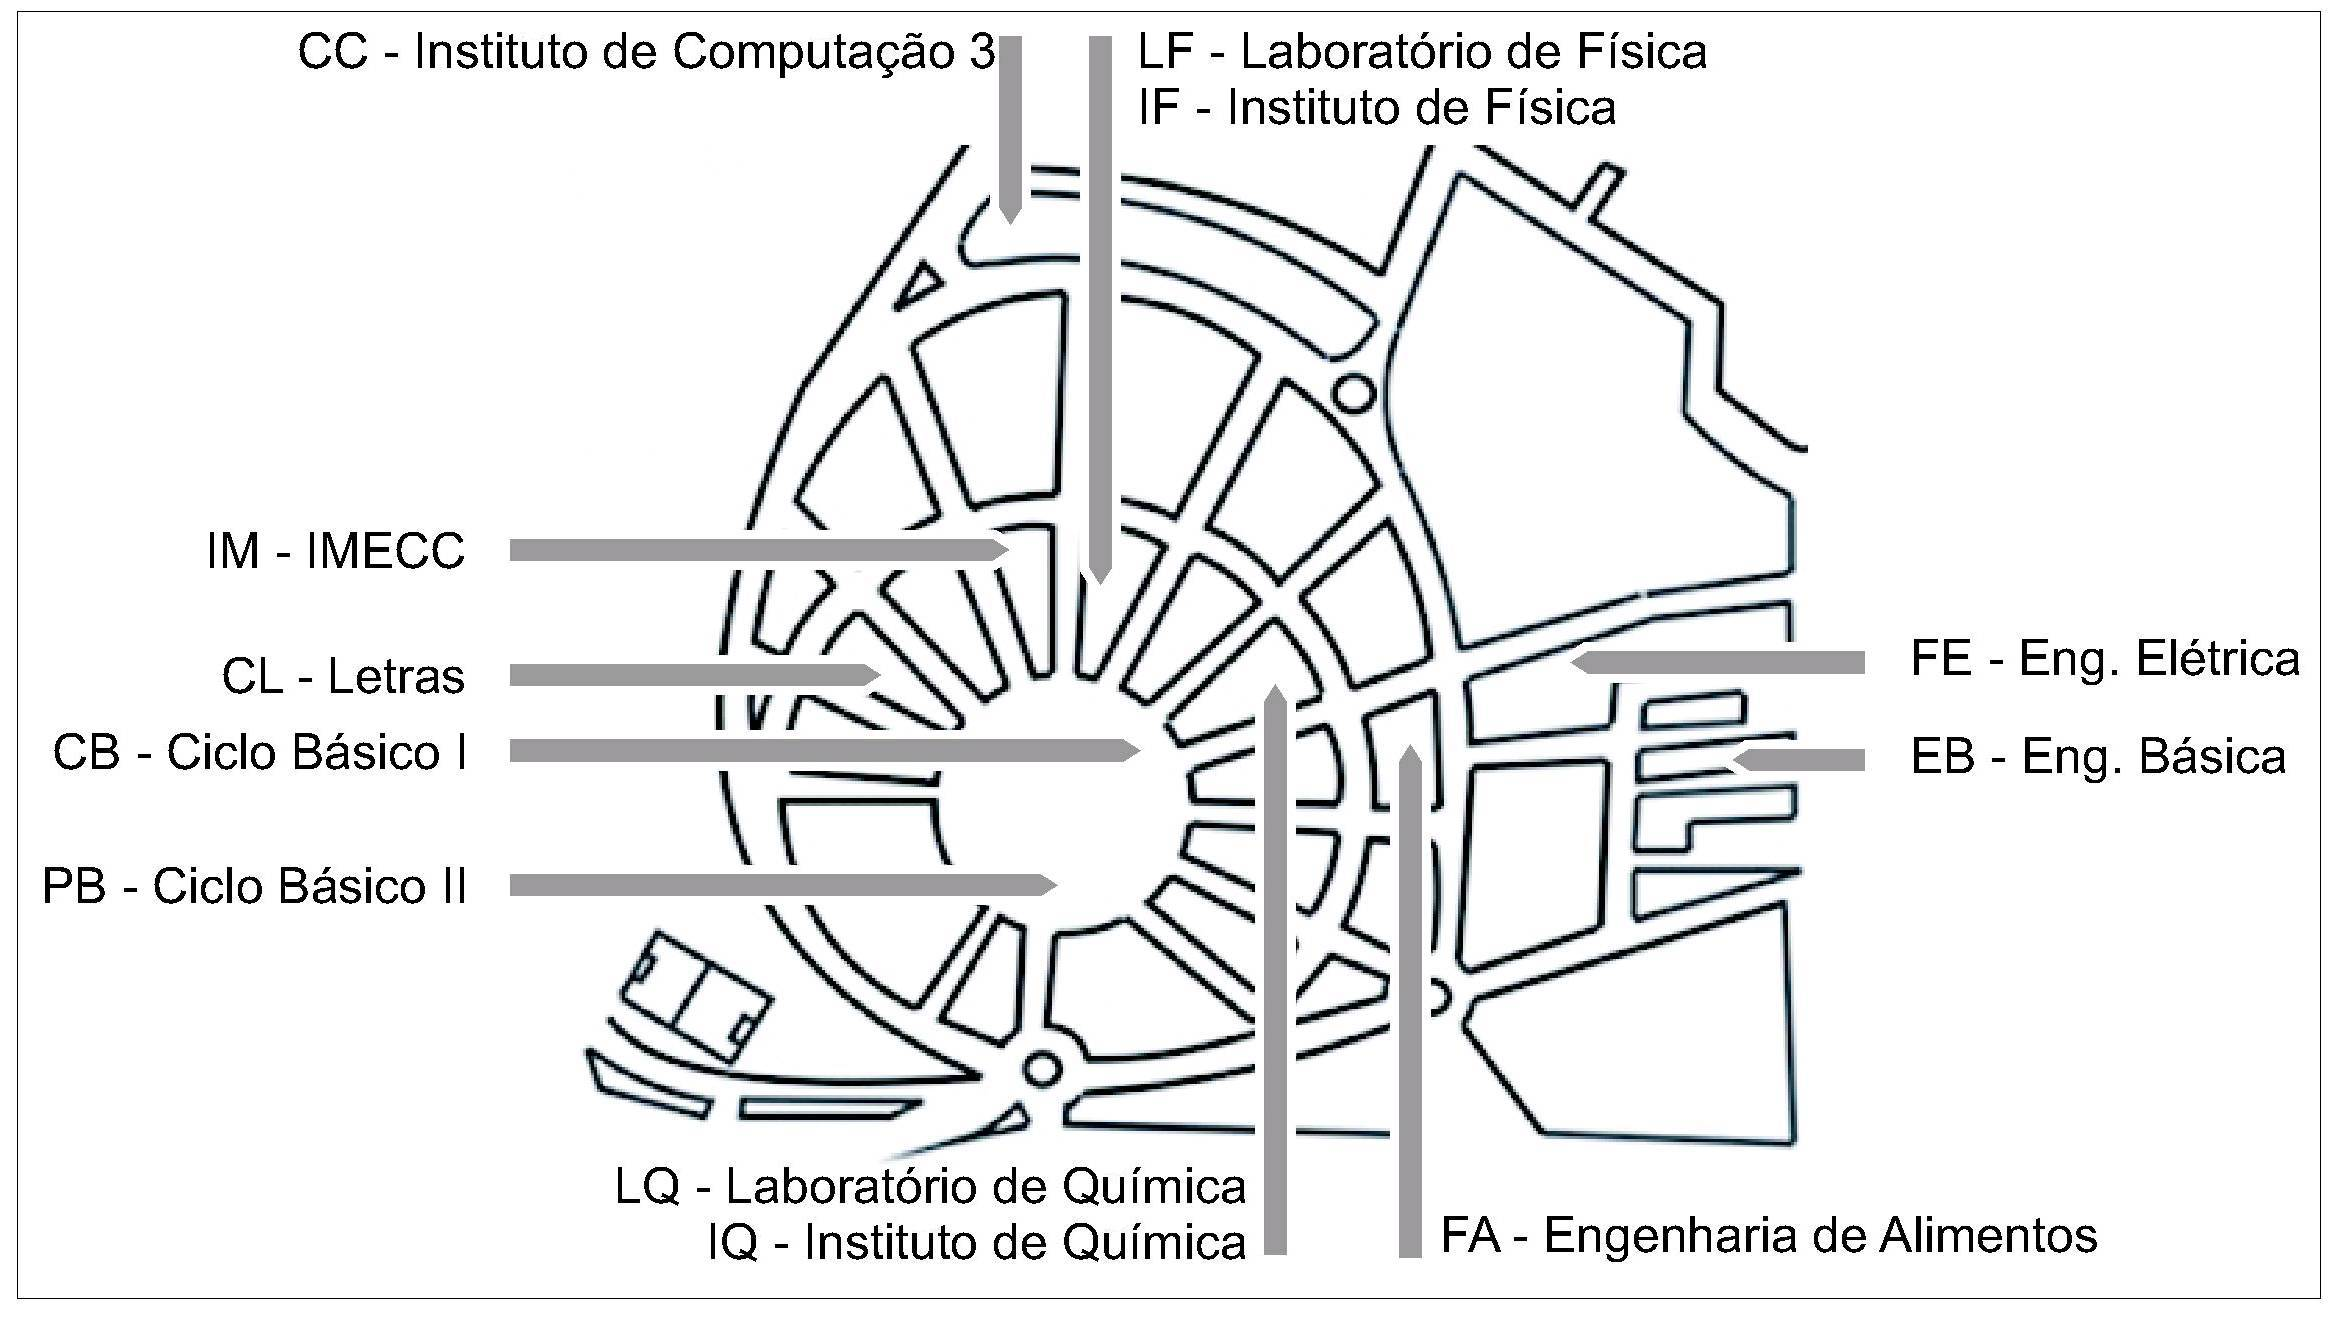
\includegraphics[scale=0.26, keepaspectratio=true]{img/imgs/10-siglas_malucas/mapa_siglas.jpg}
        \caption{Mapa com as siglas da sala de aula}
        \label{fig:mapa_siglas}
    \end{figure*}

    \item  \textbf{SAE (Serviço de Apoio ao Estudante):} É encarregado da
    execução de programas de assistência desenvolvidas pela Universidade, por
    iniciativa própria ou mediante convênios firmados com entidades
    especializadas.

    \item  \textbf{Crédito:} Unidade elementar de horas-aula de qualquer curso
    da Unicamp. Um crédito equivale a uma hora-aula semanal, ou a 15 horas-aula
    semestrais.

    \item  \textbf{Período letivo:} É um nome complicado para se referir ao
    semestre.

    \item  \textbf{Currículo pleno:} É o conjunto de disciplinas do curso que
    o aluno tem que cursar.

    \item  \textbf{CR (Coeficiente de Rendimento):} Valor entre 0 e 1 que
    é a média ponderada das notas obtidas em todas as disciplinas até o momento.
    É calculada usando como pesos o número de créditos de cada disciplina.

    \item  \textbf{CP (Coeficiente de Progressão):} É a porcentagem do curso que
    você já cumpriu. Por exemplo, se você tem CP = 0,6123 significa que você
    cumpriu 61,23\% do curso. Você se forma quando o seu CP for 1 (100\% do
    curso completo). É importante saber o CP quando for fazer algum estágio, ou
    um TCC (Trabalho de Conclusão de Curso), ou quando for cursar disciplinas
    que tenham como pré-requisito AA4xy.

    \item  \textbf{CPF (Coeficiente de Progressão Futuro):} Além do CP,
    também tem o CPF, que além do nome de um documento é o CP que você
    terá no fim do semestre caso passe em todas as disciplinas.

    \item  \textbf{CPE (Coeficiente de Progressão Exigido):} Além do CP
    e do CPF há o CPE. O CPE foi instituído a partir de 2005 e é usado
    para fins de cancelamento, ou não, de matrícula. Para que o aluno
    possa continuar a fazer o curso, ele precisa ter um CP maior ou
    igual ao CPE daquele semestre. Tanto o CP, como o CPE e o CPF
    existem somente nos cursos de graduação.

    \item  \textbf{Pré-requisito:} Matéria(s) que precisa(m) ter sido cursada(s)
    para que se possa fazer outra(s) matéria(s). Existem dois tipos de
    pré-requisitos: Os pré-requsitos totais, mais comuns, do qual é exigido
    tanto a aprovação por nota como por frequência e os pré-requisitos parciais,
    mais raros, do qual o aluno não precisa ter sido aprovado por nota, mas tem
    que ter tido aprovação por frequência e nota final maior ou igual a 3,0. Os
    pré-requisitos parciais são identificados com um asterisco na frente do
    código da disciplina (não confundir com um apontador).

    \item  \textbf{AA4xy:} Um tipo de pré-requisito. Não se trata de nenhuma
    disciplina. Para fazer disciplinas com esse pré-requisito, o aluno tem que
    tem um CP maior ou igual a 0,xy.

    \item  \textbf{AA200:} Outro tipo de pré-requisito existente, mais presente
    em disciplinas eletivas. Também não se trata de nenhuma disciplina. É apenas
    uma autorização da coordenadoria do curso. Se sobrar vagas para a disciplina
    e a coordenadoria do curso for com a sua cara você faz a disciplina.

    \item  \textbf{PB (Prédio Básico)} Também conhecido como Ciclo Básico II,
    é um prédio com várias salas de aula, que fica em frente ao Bandejão,
    e serve várias unidades que não possuem espaço físico suficiente para
    comportar seus alunos. No segundo andar ficam as salas de aula (PB01 a PB12)
    e no terceiro andar ficam os auditórios (PB13 a PB18).

    \item  \textbf{CB (Ciclo Básico I):} Tem finalidade idêntica ao PB, só que
    é muito melhor equipado, tem uma acústica muito melhor e tem um ar
    condicionado capaz de matar esquimó de frio. Fica na mesma praça que o PB,
    só que no outro extremo. À esquerda da entrada ficam as salas ímpares
    e à direita ficam as salas pares. No primeiro andar ficam os auditórios
    (CB01 a CB06) que possuem 140 e 160 lugares e no segundo andar ficam as
    salas de aula (CB07 a CB18) que possuem 60 e 80 lugares.  O CB e o PB são os
    lugares onde você vai ter a maioria das suas aulas (especialmente nos dois
    primeiros anos de curso).

\end{itemize}

\subsection{Siglas de salas de aula}

A Tabela~\ref{tab:institutos} contém algumas siglas de salas de aula que aparecem nos cadernos
de horários, disponibilizados pelas coordenadorias dos cursos e pela DAC. E a Figura~\ref{fig:mapa_siglas} aponta a localização das salas de aula pelas siglas.

\begin{center}
\begin{table*}[ht!]
{
\begin{tabular}{|l|p{6cm}|p{8cm}|}\hline

\multicolumn{3}{|c|}{ \textbf{Siglas e locais das Salas de Aula no horário}}\tabularnewline \hline

 \textbf{Sigla}  &  \textbf{Local}  &  \textbf{Referência}\tabularnewline \hline

 CB  &  Ciclo Básico I  &  Praça Central, atrás do Santander, em frente à Cantina da Física.\tabularnewline \hline

 CC  &  Instituto de Computação (IC)  &  Ao lado do Departamento de Artes Cênicas (IC-1); ao lado do IE (IC-2) e atrás do IE (IC-3).\tabularnewline \hline

 CI  &  Centro de Estudo de Línguas (CEL)  &  Atrás do IFCH.\tabularnewline \hline

 CL  &  Instituto de Estudos da Linguagem (IEL)  &  Em frente a praça central e ao lado do IFCH.\tabularnewline \hline

 EB  &  Engenharia Básica  &  Atrás da Praça da Paz e próximo à FEEC.\tabularnewline \hline

 EM  &  Faculdade de Engenharia Mecânica (FEM)  &  Atrás do IQ.\tabularnewline \hline

 FA  &  Faculdade de Engenharia de Alimentos (FEA)  &  Em frente ao IQ e à Praça da Paz.\tabularnewline \hline

 FE  &  Faculdade de Engenharia Elétrica e de Computação (FEEC)  &  Em frente à Praça da Paz.\tabularnewline \hline

 IB  &  Instituto de Biologia (IB)  &  Entre o IQ e o Serviço Social do SAE.\tabularnewline \hline

 IE  &  Instituto de Economia (IE)  &  Atrás do IMECC.\tabularnewline \hline

 IF  &  Instituto de Física (IFGW)  &  Em frente ao Ciclo Básico, e a Química.\tabularnewline \hline

 IH  &  Instituto de Filosofia e Ciências Humanas (IFCH)  &  Entre o IMECC e o IEL.\tabularnewline \hline

 IM  &  Instituto de Matemática, Estatística e Computação Científica (IMECC)  &  Em frente a Praça Central.\tabularnewline \hline

 IQ  &  Instituto de Química (IQ)  &  Entre o IB e o IFGW.\tabularnewline \hline

 LE  &  Laboratórios de informática da FEEC  &  Em frente a Praça da Paz e ao lado das salas de aula da FEEC.\tabularnewline \hline

 LF  &  Laboratório de Física  &  Em frente à cantina do IMECC.\tabularnewline \hline

 LQ  &  Laboratório de Química  &  Em frente à biblioteca do IQ.\tabularnewline \hline

 PB  &  Ciclo Básico II, Prédio Básico  &  Praça Central, em frente ao Bandejão.\tabularnewline \hline

\end{tabular}
}
\hfill{}
\caption{Siglas das salas de aula}
\label{tab:institutos}
\end{table*}
\end{center}

\section{Disciplinas}

\subsection{Matrícula}

A Unicamp é muito diferente da sua escolinha onde a tia Gertrudes entregava
o seu horário impresso coloridinho para você colar na capa do seu fichário.
À exceção do primeiro semestre letivo, no qual você já entra matriculado em
todas as matérias obrigatórias, na Unicamp você vai ter que se virar.  O GDE
(\url{www.gde.ir}) é uma ferramenta criada por um aluno da Engenharia e adotada
pela DAC que facilita muito o planejamento do seu horário, além de servir como
uma rede social interna.

Peça sempre a ajuda dos seus veteranos quando for montar seu horário. Informe-se
sobre todos os professores que oferecem as matérias, se eles são coxas ou
carrascos, bons ou ruins, se demoram para entregar as notas{\dots} Você vai
poupar muita dor de cabeça. O melhor lugar para essas discussões é o grupo de
e-mail da sua turma.  Pode ter certeza que ela terá um assim que você entrar na
Unicamp.

\subsection{Cancelamento, Trancamento e Desistência}

Embora praticamente todos os alunos da Unicamp usem esses três termos
indiscriminadamente, como se fossem sinônimos, para a DAC, esses três termos têm
significados bastante distintos. Aí vai o que cada termo significa:

\begin{itemize}
\item Desistência de matrícula em disciplinas
      (\url{www.dac.unicamp.br/portal/grad/regimento/capitulo_iii/secao_v/index.html}):
      Processo que é chamado pelos alunos de "trancamento".
      O aluno não mais cursa essa disciplina no semestre,
      tendo de cursá-la em algum semestre posterior. Só é possível desistir uma vez da
      disciplina e pode-se pedir desistência até que se tenha passado metade do
      semestre.
\item Cancelamento de matrícula
      (\url{www.dac.unicamp.br/portal/grad/regimento/capitulo_iii/secao_vii/index.html}):
      Processo em que o aluno se desliga da Unicamp, por motivo de jubilação, por
      ter faltado às duas primeiras semanas do ano de ingresso, por ter sido
      reprovado em todas as disciplinas do primeiro ou do segundo semestre de
      ingresso, por ter sido expulso, por ter sido aprovado em outra universidade
      pública (não é permitido fazer mais do que um curso de universidade pública
      simultaneamente), ou por vontade própria do aluno.
\item Trancamento de matrícula
      (\url{www.dac.unicamp.brportal/grad/regimento/capitulo_iii/secao_vi/index.html}):
      Processo em que o aluno não cursa qualquer disciplina da Unicamp durante
      o semestre. O aluno tem direito a fazer até dois trancamentos de matrícula, em
      semestres seguidos ou não e o aluno não pode trancar nenhum dos dois
      semestres do ano de ingresso. Desistência de todas as disciplinas
      configura-se como trancamento. O trancamento é pedido na DAC, e pode ser
      pedido até que se tenha transcorrido 2/3 do semestre (geralmente de dezembro
      até fim de maio para trancamento de primeiro semestre; e de julho até fim de
      outubro para trancamento de segundo semestre). Para cada trancamento,
      o prazo máximo de integralização é postergado.
\end{itemize}

\subsection{Eletivas e Teste de Proficiência}

A Unicamp oferece a seus alunos a oportunidade de personalizar seu currículo de
acordo com seu interesse por meio das \textbf{disciplinas eletivas}. Ao contrário das
disciplinas obrigatórias, com as eletivas você pode escolher a matéria que vai cursar. Alguns
créditos podem ser cumpridos com qualquer disciplina oferecida pela
Universidade, outros estão restritos a um determinado conjunto. Para mais
detalhes, consulte seu catálogo em
\url{www.ic.unicamp.br/graduacao/catalogos-de-graduacao}.

Mas não se esqueça de que com um grande poder vem uma grande responsabilidade!
A Unicamp lhe dá liberdade para escolher o melhor jeito de se preparar para seu
futuro, e espera que você saiba o que fazer com essa liberdade. Você pode socializar com
outros cursos, aprender uma língua estrangeira, assistir a seminários ou obter
um certificado de estudos na FEEC ou no IC.

\textbf{Teste de proficiência} é uma prova que permite dispensa de cursar uma disciplina
(desde que você obtenha a nota mínima, é claro). Se você acha que sabe o suficiente
sobre eletromagnetismo, por exemplo, pode tentar a proficiência de Física Geral III.
Nem todas as disciplinas oferecem o teste, e você só pode fazê-lo uma vez por
disciplina -- e se você já se matriculou na disciplina e não passou, não pode fazer.
Além disso, fazer o teste de proficiência também é obrigatório para se matricular
nas disciplinas de língua inglesa e japonesa, independentemente de conhecimento
prévio na língua.

Fique ligado no calendário da DAC para não perder as datas de inscrição nos
testes de proficiência! As datas dos testes de línguas são sempre no começo do
ano, diferentes das demais, que são no fim de cada semestre.

Disciplinas eletivas e teste de proficiência estão relacionados porque muitas pessoas,
especialmente nos cursos de computação, fazem proficiência em
disciplinas de línguas, eliminando créditos de eletivas, em alguns casos para evitar o jubilamento, outros para não ter que
passar mais um semestre na faculdade. Apesar de registrar a familiaridade do
aluno com uma outra língua em sua integralização, essa prática não enriquece
a graduação de nenhum estudante que faça tal escolha. Além disso, muitos bixos
arrependem-se de terem feito a prova e perdido preferência na hora de pegar uma
disciplina interessante, podendo até mesmo não conseguir se matricular. Isso acontece
porque, depois que seus créditos de eletivas se esgotam, você começa a puxar matérias
não-obrigatórias como \textbf{extracurriculares} e tem prioridade menor na
atribuição de vagas.

Converse com seus amigos e veteranos para descobrir o melhor jeito de usufruir
dessa liberdade que poucas universidades oferecem! Dificilmente você não
encontrará algo com o qual se identifica ou que não ensine lições interessantes.

Para mais informações sobre teste de proficiência, acesse:
\url{www.dac.unicamp.br/portal/grad/avaliacao_e_frequencia/teste_de_proficiencia/}.

\subsection{Avaliações de professores}

Achou que o professor ensinou muito mal? Ele falou da vida, do universo e tudo
mais -- menos sobre a disciplina? Foi incoerente? Ou, pelo contrário, achou o
professor o máximo e a sala do CB a oitava maravilha do mundo? Não adianta
xingar nem elogiar no Twitter!

Nas últimas aulas de cada semestre, todos os professores devem disponibilizar um
formulário de avaliação. Esse é o momento para que você possa separar os acertos
dos erros, portanto preencha com seriedade. Os dados serão analisados pelas
Comissões de Graduação de cada unidade e os comentários escritos serão repassados
para o professor.

Além dos formulários, a PRG (Pró-reitoria de Graduação) realiza o Programa de
Avaliação da Graduação no fim de cada semestre. Trata-se de uma pesquisa on-line
semelhante aos formulários de cada unidade, porém unificada para toda a Unicamp
e mais abrangente em suas perguntas.

O GDE (\url{gde.ir}) também tem um sistema de avaliação de professores, cuja nota
costuma ser usada pelos alunos como um dos critérios no momento de decidir com
que professor puxar uma matéria.

Durante o semestre, ocorre a Reunião de Avaliação de Curso. A data e o horário
serão divulgados pelas unidades e pelo CACo. Essa é uma oportunidade de passar
para as coordenadorias do curso não só suas impressões sobre professores e disciplinas,
mas sobre qualquer assunto relacionado ao curso. Antes da Reunião, o CACo também
promove um PipoCACo de Avaliação de Curso, motivando uma pré-discussão.

Tenha sempre em mente que a nossa percepção sobre o oferecimento de uma disciplina
não é óbvia para os professores. Preencha todas as avaliações com sinceridade
e use sempre os espaços dedicados a comentários. Além disso, cultive o hábito de
realizar uma avaliação informal do professor no fim de cada semestre -- mandando
um e-mail, por exemplo. O valor deste tipo de avaliação é muito grande.

\newpage
\section{Lugares para estudar}

Há vários lugares para estudar na Unicamp. Você pode escolher o que você achar
melhor:

\begin{itemize}
    \item  \textbf{Biblioteca Central (BC):} A BC tem três andares. O primeiro
    é onde tem os livros gerais e onde a galera estuda. Geralmente é barulhento em
    épocas de provas, mas é bom porque sempre tem lugar para estudar e fecha às 22h.
    Se você não se importa com barulho, ou até acha que você faz bastante, esse
    é o lugar da BC para você estudar. O segundo andar é onde está a BAE,
    a Biblioteca da Área de Engenharia. Um pouco mais silenciosa que a BC nas mesas
    externas, esse andar tem salas para estudo em grupo, bastante silenciosas, mas
    que sempre estão ocupadas em época de provas, e mesas individuais escondidas
    entre os periódicos. O terceiro andar é para silence freaks. Morbidamente
    silencioso, desértico (muita gente desconhece a existência desse andar), esse
    é o lugar mais silencioso da BC para estudar. Tem umas salinhas de estudo
    individual e duas mesas para estudo em grupo. O problema é que fecha às 17h, mas
    o pôr-do-sol de lá de cima também é ma-ra-vi-lho-so.

    \begin{figure}[h!]
        \centering
        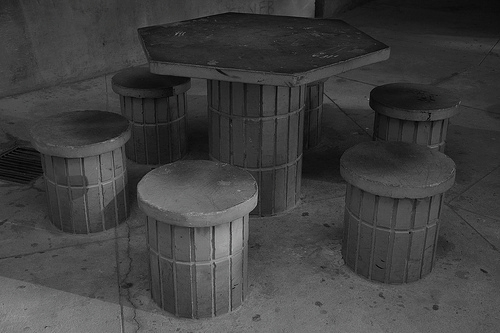
\includegraphics[scale=0.60, keepaspectratio=true]{img/imgs/11-lugares_estudar/-072.jpg}
    \end{figure}

    \item  \textbf{Arcádia (ou mesinhas do IEL):} A Arcádia é algumas mesas ao ar
    livre no IEL (Instituto de Estudos da Linguagem). Em horários de aula
    é silencioso, é um ambiente muito agradável e por ser ao ar livre, não fecha.
    Tem dois problemas: O grande fluxo de pessoas no local pode facilmente
    distraí-lo, principalmente se você as conhecer, e à noite enche de insetos (além
    da iluminação não ser das melhores). Às vezes, venta bastante e é ruim para
    estudar com folhas avulsas. Mas ainda assim é um ótimo local para estudar.

    \item  \textbf{Biblioteca do IFGW:} A biblioteca do IFGW (Instituto de Física
    Gleb Wataghin) é ótima para dias de calor, por ser super gelada (ar-condicionado
    mega-super-power!). Tem vantagem sobre as outras bibliotecas pelo fato das salas
    de estudo serem fora da biblioteca e por isso você não precisa deixar o seu
    material para entrar na sala de estudos. Recentemente reformada, agora conta
    com 6 baias para estudo em grupo e quantidade razoável de baias individuais, com tomadas
    onde você pode plugar seu notebook.

    \item  \textbf{BIMECC:} A biblioteca do IMECC tem poucos lugares, poucas
    mesas para estudo individual, os locais de estudo ficam dentro da biblioteca
    (você precisa guardar sua bolsa para entrar), não é muito gelada
    e o ambiente não é agradável, mas nela e na BAE é que você encontrará
    a maioria dos livros relacionados a computação.

    \item  \textbf{Outras bibliotecas:} Aventure-se por outras bibliotecas, como
    a da Economia, a da Pedago e a da Biologia e as conheça. Para aqueles que
    gostam (ou são obrigados) a estudar aos fins de semana a BC e as bibliotecas
    da Educação, da Economia, da Química, da Medicina, do IEL e da Geociências
    abrem aos sábados. Para saber os horários de funcionamento das bibliotecas,
    entre no site do SBU (\url{www.sbu.unicamp.brindex.php?link=30}).

    \item  \textbf{Bitolódromos:} Existem dois bitolódromos na Unicamp: O do IC
    e o da FEEC (coincidência interessante, né?). O do IC-3 é uma mesa grande
    com algumas cadeiras no corredor dos laboratórios. O da FEEC fica no fundo do
    prédio principal (qualquer veterano sabe onde é o bitolódromo, não tenha
    vergonha de perguntar). O da FEEC é maior, você se distrai menos porque não
    estão todos os seus colegas (mas várias outras pessoas estão) entrando
    e saindo de lá (embora os pica-fios sejam bastante barulhentos), e sempre
    você encontra gente que possa te ajudar. O do IC serve para quando você já
    estiver lá e com preguiça de ir à Elétrica, porque o da FEEC é muito melhor.

    \item  \textbf{Sala 316:} Outro alento para as madrugadas de estudo é a sala
    316 do IC-3, que fica aberta sempre, ou então, aberta facilmente com a chave
    em posse do guardinha. É uma sala com carteiras legais, lousa e ar
    condicionado, aliás, é muito boa para estudo em grupo (NABVS IMINENTVS) por
    causa da lousa.

    \begin{figure}[h!]
        \centering
        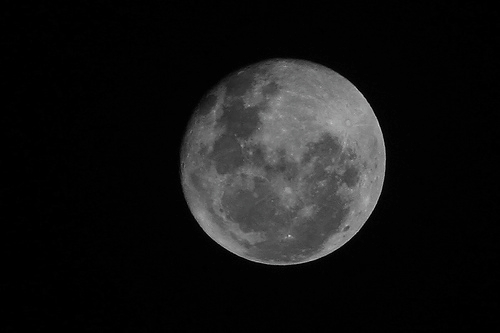
\includegraphics[scale=0.50, keepaspectratio=true]{img/imgs/11-lugares_estudar/-076.jpg}
    \end{figure}

    \item  \textbf{Sala 363:} Vulgo salinha de estudo do IC. Pequena
    e aconchegante, tem mesas redondas, muito boas para estudo em grupo. Não
    costuma encher, por isso é bem tranquila. Tem uma estante com vários livros
    doados para uso livre.

    \item  \textbf{Sua casa:} Se você mora em uma república com pessoas da sua
    turma, vá fundo e estude em casa. Se você mora sozinho ou com caras de
    outros cursos/anos, mas se concentra bem em casa, também o faça. Caso
    contrário, estude na Unicamp. É muito fácil se distrair em casa. Você vai
    à geladeira, mexe no computador, lê outra coisa, deita na cama e dorme,
    entre outras coisas. Prefira estudar na Unicamp. Outra coisa, não seja
    egoísta, quando tiver oportunidade de estudar em grupo, prefira essa
    alternativa. Lembre-se que você não está mais no "cursinho", tente sempre
    pegar as dicas que a galera te dá, principalmente dos seus veteranos.
\end{itemize}

\newpage
\section{Melhores banheiros}

Uma das maiores necessidades do ser humano pode ser potencializada se for
realizada num banheiro decente. Portanto, é muito importante que você saiba onde
ir. Alguns dos melhores banheiros da Unicamp são:

\begin{itemize}

    \item  \textbf{IC-3:} Geralmente estão limpos e utilizáveis. Mas fedem!
    Sempre com papel higiênico, é uma boa pedida na hora do apuro. Exceto nos
    finais de semana.

    \item  \textbf{IC-2:} Quase sempre estão limpos e utilizáveis e tem um odor
    melhor que os do IC-3. Só precisa tomar cuidado pois, as vezes, falta papel
    higiênico.

    \item  \textbf{FEEC:} Possui excelentes banheiros escondidos por lá. Procure
    bem!

    \item  \textbf{PB:} Os banheiros do segundo e do terceiro andar do Pavilhão
    Básico também são bons (especialmente os do terceiro andar, por quase não
    serem usados). Só tome cuidado, porque às vezes não tem papel higiênico.

    \begin{figure}[h!]
        \centering
        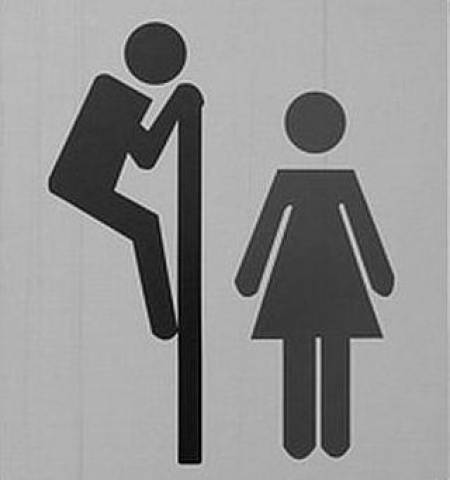
\includegraphics[scale=0.50, keepaspectratio=true]{img/imgs/12-melhores_banheiros/banheiro.jpg}
    \end{figure}

    \item  \textbf{FE:} A faculdade de educação tem poucos banheiros masculinos,
    mas estão entre os melhores da Unicamp pelo pouco uso.

    \item  \textbf{CB:} Estes banheiros ficam escondidos próximo às escadas do
    CB (no térreo). Se você tiver sorte de chegar bem após a limpeza, o banheiro
    estará em excelentes condições. Porém, na maior parte do tempo ele fica bem
    sujinho.

    \item  \textbf{DEQ:} Departamento de Eletrônica Quântica, no IFGW. Dizem que
    ninguém os usa.

    \item  \textbf{DRCC:} Departamento de Raios Cósmicos e Cronologia, no IFGW.
    Um dos melhores banheiros existentes na Unicamp (senão o melhor). Assim como
    os banheiros do DEQ, dizem que ninguém os usa.

    \item  \textbf{DFA:} Departamento de Física Aplicada, no IFGW. Os dois
    andares do departamento tem banheiros bons e utilizáveis, mas algumas vezes
    falta papel higiênico.

    \item  \textbf{IMECC:} Todos os três departamentos (andares) do IMECC tem
    banheiros bons e utilizáveis. Mas vez ou outra falta papel higiênico.
\end{itemize}
